% This is samplepaper.tex, a sample chapter demonstrating the
% LLNCS macro package for Springer Computer Science proceedings;
% Version 2.20 of 2017/10/04
%
\documentclass[runningheads]{llncs}
%
\usepackage{graphicx}
\usepackage{float}

% Used for displaying a sample figure. If possible, figure files should
% be included in EPS format.
%
% If you use the hyperref package, please uncomment the following line
% to display URLs in blue roman font according to Springer's eBook style:
% \renewcommand\UrlFont{\color{blue}\rmfamily}

\begin{document}
%
\title{Occupational Strain and Coronary Heart Disease: a Bayesian Network Analysis}
\titlerunning{Occupational Strain and Coronary Heart Disease: a BN Analysis}
%
%\titlerunning{Abbreviated paper title}
% If the paper title is too long for the running head, you can set
% an abbreviated paper title here
%

% First names are abbreviated in the running head.
% If there are more than two authors, 'et al.' is used.
%
\institute{Vrije Universiteit Amsterdam, De Boelelaan 1105, 1081 HV Amsterdam,\\ The Netherlands}
%
\maketitle              % typeset the header of the contribution
%
\begin{abstract}
%A Bayesian Network (BN) is a probabilistic graphical model for representing dependencies and conditional independencies of given propositional variables that belong to a specif domain. 
%In the current paper we will discuss the implementation of a BN Reasoner, which contains a set of functionalities to test the network, with different heuristics and given the following problem statement: given the correlation between occupational strain, work-related stress, and coronary heart disease, which variables come into play to affect the correlation? 
A Bayesian Network (BN) is a tool for representing probabilities of events and their interaction. In this paper, we present a BN Reasoner that contains functionality to query information from a BN and we assess the performance of different ordering heuristics in variable elimination. The minimum degree and minimum fill heuristics both performed similarly and significantly outperformed random ordering. 
Then we consider the use case of investigating the correlation between occupational strain, work-related stress, and coronary heart disease (CHD), by modelling their probabilities and interactions through a BN. This network is then queried and the results are compared with insights from medical research. We found that if a person is a heavy smoker and has a high job demand, he or she is more likely not to develop CHD than to develop it. Furthermore, the most likely instantiation of a person with high cholesterol and hypertension is someone who is also male, and scores true on all risk variables apart from the occupational strain (OS). When there is OS and limited social opportunities, our findings suggest that it is most likely to be a man with an active job type (JT). Given the evidence of both OS and Mobbing, the d-separation indicated true is independent of gender and JT.

\keywords{Bayesian Network \and Minimum degree \and Minimum fill \and Random Ordering \and Occupational Strain \and Coronary Heart Disease}
\end{abstract}
%
%
%
\section{Introduction}

Cardiovascular disorders continue to be a major cause of death in the Western world. Along with all the studied physical risk factors of Coronary Heart Disease, researchers have also examined the role of psychological factors, such as personality type and psychological stress. Job strain, definable as work environment-related stress, is one of the most widely studied aspects of psycho-social stress and its importance as a risk factor for coronary heart disease remains controversial. According the World Health Organization, occupational strain is a response employees develop when presented with work demands and pressures that they are not able to cope with.  
With the aim of investigating the correlation between occupational strain and the incidence of coronary heart disease, a Bayesian Network (BN) was used to establish a framework of fourteen probabilistic variables with interactions between them. %wanna write the hypothesis
A BN is a form of statistical modeling which allows us to obtain a graphical network describing the dependencies and conditional probabilities of given propositional variables from empirical data. They have proven to be an effective tool for capturing the relationships between the factors belonging to a defined domain. 
In the upcoming sections we will describe the implementation of the BN Reasoner and the evaluation of its performance, a detailed explanation of our network, the hypothesis tested and a final discussion. 

\section{The Bayesian Network Reasoner}
\label{BNReasoner}

A Bayesian Network (BN), as stated above, is a probabilistic graphical model where each node corresponds to a random variable and each edge represents the conditional probability for the corresponding variables. A BN corresponds to a directed acyclic graph (DAG) and to a set of conditional probability tables (CPTs), which, for every value \textbf{x} of variable \textbf{X} and every instantiation \textbf{u} \textbf{U}, define the Pr(\textbf{x}$\mid$\textbf{u}). 

\intextsep
\begin{figure}[H]
    \centering
    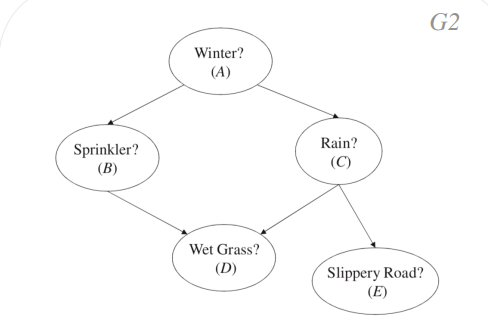
\includegraphics[width=0.45\textwidth]{Assets/BN example1.png}
    \hfill
    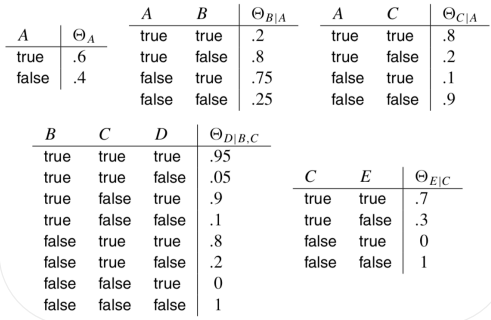
\includegraphics[width=0.45\textwidth]{Assets/BN example2.png}
    \caption{BN example}
    \label{fig:my_label}
\end{figure}

The Bayesian Network Reasoner has been implemented using the following algorithms:

\subsubsection{d-Separation:} %The structure of a Bayesian Network is interpreted as declaring a number of independence statements and probabilistic independence satisfies the graphoid axioms. 
One can derive new independencies to the independencies declared in the structure using d-separation. According to d-separation variable \textbf{X} are d-separated from variable \textbf{Y} by variables \textbf{Z} if every path from node \textbf{X} to node \textbf{Y} is blocked by \textbf{Z}. \textbf{X} and Y are d-separated by \textbf{Z} in DAG \textit{G} if and only if the graphoid axioms can be used to show that \textbf{X} and \textbf{Y} are independent given \textbf{Z}.  
\\
This graphical test was implemented by first pruning (i.e. deleting) all leaf nodes in the graph that are not part of the union of \textbf{X}, \textbf{Y} and \textbf{Z}. Then all edges outgoing from the variables in \textbf{Z} are removed. Finally, a recursive function iterates through all variables in X and their neighbours and calls itself for every neighbour while keeping track of the variables that have been visited in a set, these are skipped. It returns $True$ when it comes across a variable in \textbf{Y}, since this means that \textbf{X} and \textbf{Y} are connected, otherwise it returns $False$ when it has iterated through all variables connected to \textbf{X}. The output of the d-seperation function is then the opposite of the aforementioned recursive function, since two variables are d-seperated by Z when they are not connected after the pruning steps mentioned above.

\subsubsection{Ordering:} In solving a query, we apply variable elimination to remove the variables which are not relevant to answer the query. Given an interaction graph \textbf{G} and variable \textbf{X} to eliminate, we obtain \textbf{G'} adding an edge between every pair of neighbours of \textbf{X} that are not already connected by an edge, we delete \textbf{X} from \textbf{G}, multiply all factors containing \textbf{X} and finally sum-out \textbf{X} from the resulting factor. The order in which variables are eliminated is important and two heuristics can be used: 

\paragraph{min-degree:} always choose the node with the smallest degree. The way that this has been implemented is by creating the interaction graph of the network and iterating through each node while counting the number of edges and adding the node with the smallest number (which is the degree) to the list. 

\paragraph{min-fill:} always choose the node whose elimination adds the smallest number of edges. The implementation of this function first creates an interaction graph of the network and then computes for each node how many edges would be added if this node were to be deleted (this is done by counting how many of the node's parents are not connected to each other). The node with the lowest value is then added to the list.

\subsubsection{Network Pruning:} Network pruning is done through Node Pruning and Edge Pruning. With node pruning, given a BN \textbf{N} and a query (\textbf{Q,e}), we can remove any leaf node from \textbf{N} as long as it does not belong to variables \textbf{Q U e}. With edge pruning, for each edge from node \textbf{U} to \textbf{X}, we can remove the edge from \textbf{N} and replace the CPT of $\Theta$X $\mid$ U by a smaller CPT obtained from  $\Theta$X $\mid$ U assuming the value \textit{u} of \textbf{U} given in evidence \textit{e}.

\subsubsection{Marginal Distributions:} Given two variables \textbf{X} and \textbf{Y}, their marginal distribution is their joint probability distribution. We define \textbf{prior marginal} as our prior belief about the value of variable \textbf{X}, while we refer to \textbf{posterior marginal} as our knowledge about variable \textbf{X} having observed variable \textbf{Y}. 

\subsubsection{MAP and MPE:} MAP (Most a Posteriori Hypothesis) and MPE (Most Probable Explanation) refers to two types of queries representing the most likely instantiations (i.e. truth value assignments) of the variables in the network. 
%MAP queries refers to the most likely instantiation of variables given the evidence. MPE queries consider the most likely instantiation of the variables excluding the evidence. 
While both MAP and MPE compute this query based on evidence (given variable assignments), MAP focuses on a subset of variable instantiations, while MPE computes the most likely assignment of each variable.
The specific method for eliminating a variable depends on the query, for example, to solve the condition probability the variables have to be summed out. To solve an MPE problem we eliminate the variables by maxing them out while a MAP query requires both summing-out and maxing-out.   










\section{Performance Evaluation}
\label{Testing}

After implementing the aforementioned tasks, we run an experiment in order to test the average performance of the MAP and MPE algorithm with three different elimination order algorithms; the random order, the min-order and min-fill heuristics described in Section \ref{BNReasoner}. The metrics used to evaluate the results are the following:
\begin{itemize}
    \item Run time
    \item Number of nodes
    \item Tracked degrees throughout the execution
\end{itemize}
The experiment has been run ten times per heuristic for each algorithm, and the average of those runs is presented in the later plots for each metric.

\subsection{Experiment Preparation}
We created a script that generates different Bayesian networks to implement the experiment. Each implemented network has two root nodes and a minimum number of five variables, while every child has a minimum of one parent and a maximum of three. During the experiment, each generated network grew by ten nodes each time. A total number of five networks was created and used for this experiment. 
Regarding the queries, we chose to have the same ratio of given evidence and map variables in the five Bayesian Networks mentioned above, aiming to compare the performance of the implementation independently of the given parameters. For both queries, the ratio of given evidence equals $2.5$, i.g a five-node BN corresponds to $5/2.5$ evidence, while a fifteen-nodes BN to six given evidence. The same logic stands for the MAP variables ratio used in the MAP queries, which equals $2$. The variables selected as evidence cannot be chosen as MAP variables.

\subsection{Results}
As shown in Figure \ref{fig:time_nodes}, the two heuristics generally outperform the random order in both MPE and MAP queries. The first graph shows that all three elimination order functions run approximately the same time between five and fifteen nodes. However, from twenty-five nodes onwards, the two heuristics perform roughly the same as before, while the random order grows exponentially.\\
Regarding the second graph of the figure, the run time for a MAP query is illustrated. As can be seen, the number of nodes and the run time increase accordingly, with the random order requiring the most time once again. The difference is not as noticeable as in the previous graph, but it is still significant.

\intextsep
\begin{figure}[H]
    \centering
    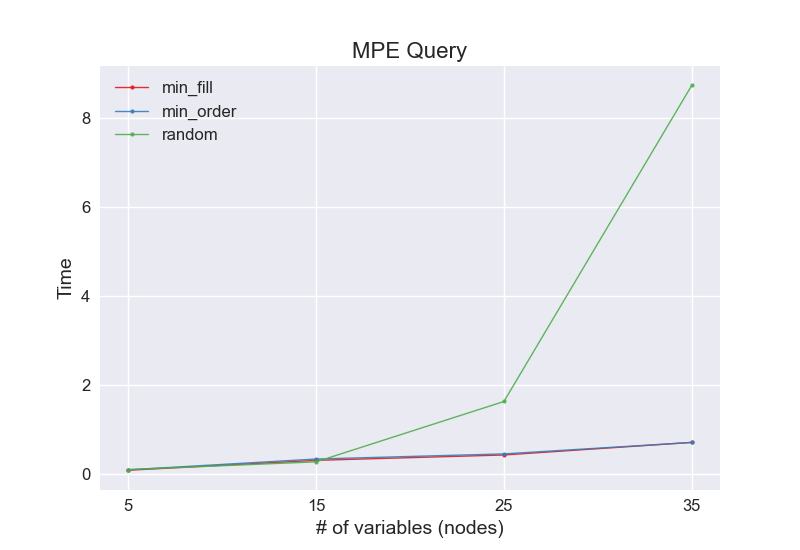
\includegraphics[width=0.45\textwidth]{Assets/mpe_query.png}
    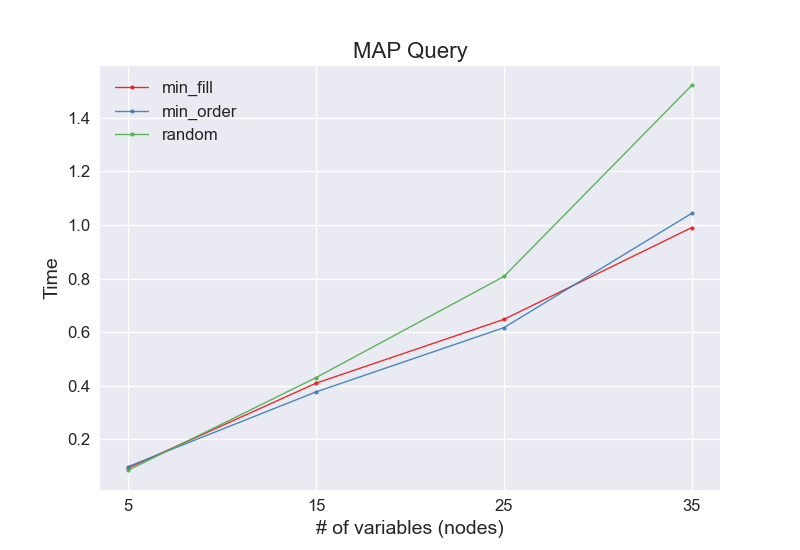
\includegraphics[width=0.45\textwidth]{Assets/map_query.png}
    \caption{Number of nodes vs. Time}
    \label{fig:time_nodes}
\end{figure}\\



To evaluate further the different orderings,  we tracked the degrees of each order during the execution of the queries. In other words, every time an elimination occurred in the algorithm, we counted the number of variables included in the newly created factor. This number corresponds to the width of the used order π and is a way to measure the order quality. In the figures \ref{fig:mpe_histograms} and \ref{fig:map_histograms}, three different histograms are illustrated per query, and each histogram represents how many times each degree occurred in the five, twenty-five and forty-five BNs, respectively.

The different degrees tracked in the MPE Queries are shown in Figure \ref{fig:mpe_histograms}. Based on the graphs, the degrees occurred using the heuristics overlap in all tested BNs independently of the variable size and fluctuate in a smaller scale than random order. The histogram correlates perfectly with the line plot in Figure \ref{fig:time_nodes}.

\intextsep
\begin{figure}[H]%
    \centering
    \subfloat[\centering a ]{{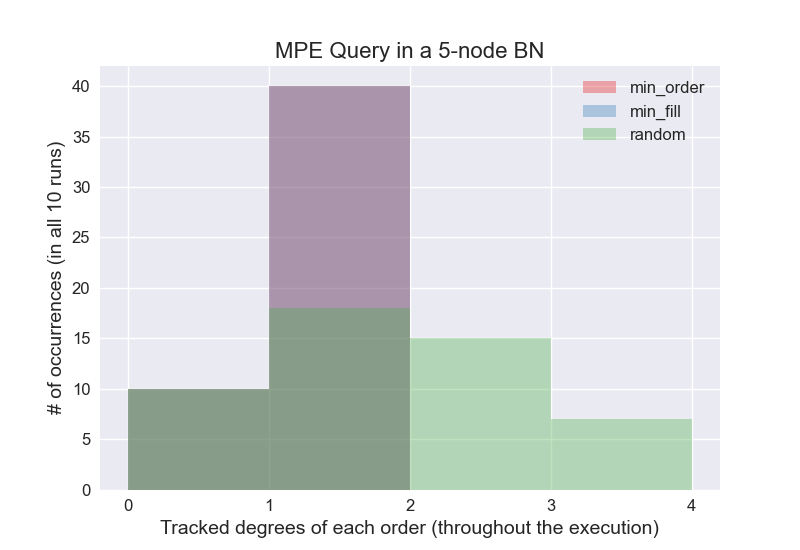
\includegraphics[width=5.2cm]{Assets/mpe-hist.png} }}%
    \qquad
    \subfloat[\centering b ]{{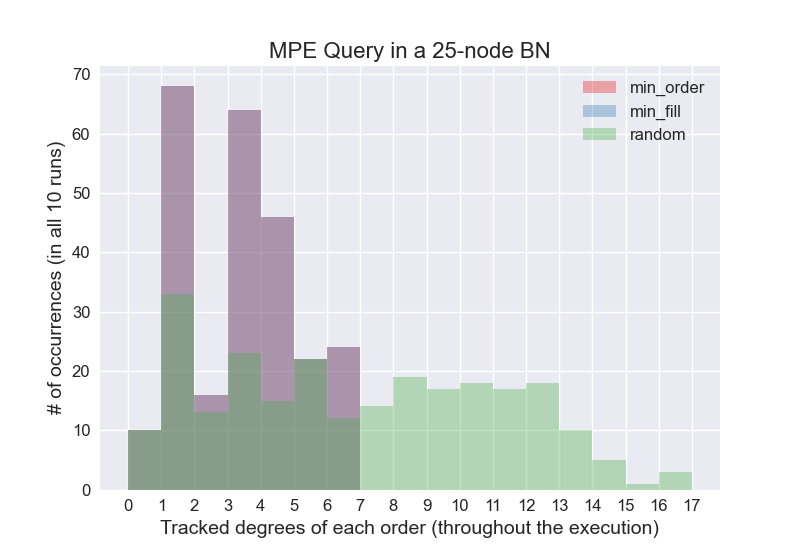
\includegraphics[width=5.2cm]{Assets/mpe-hist-25nodes.png} }}%
    \qquad
    \subfloat[\centering c ]{{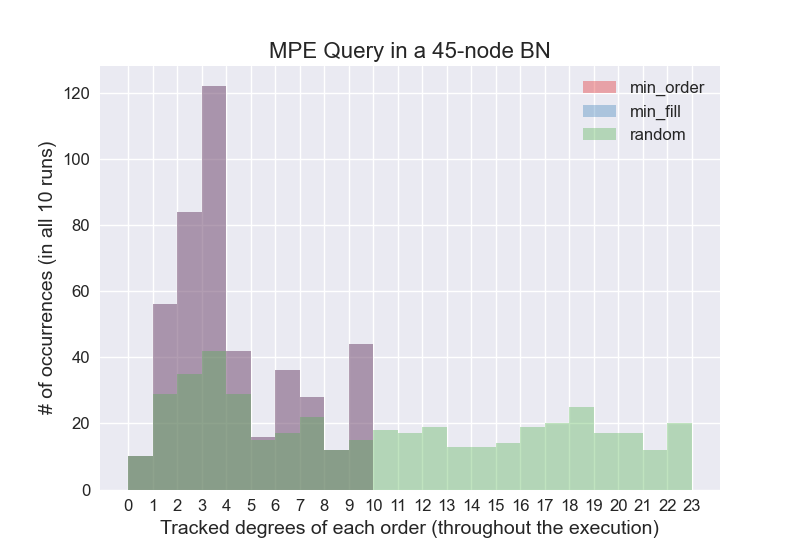
\includegraphics[width=5.2cm]{Assets/mpe-hist-45nodes.png} }}%
    \qquad
    \caption{MPE Queries}%
    \label{fig:mpe_histograms}%
\end{figure}

On the other hand, in Figure \ref{fig:map_histograms}, the degrees of the two heuristics do not match for more than twenty-five node BNs when executing the MAP queries. Nevertheless, the width fluctuates in a similar scale with min-fill to perform slightly better than the min-order heuristic. Regarding the random orderings, the width reaches higher numbers than the other two methods.

\intextsep
\begin{figure}[H]%
    \centering
    \subfloat[\centering a ]{{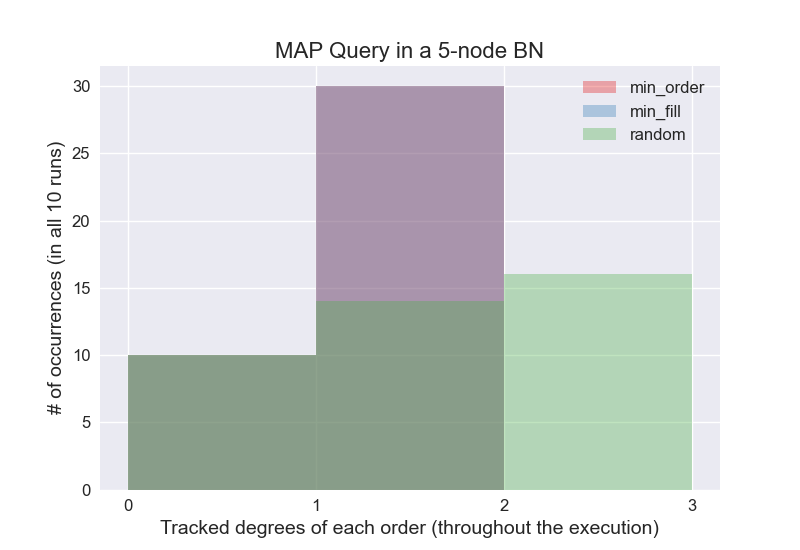
\includegraphics[width=5.2cm]{Assets/map-hist.png} }}%
    \qquad
    \subfloat[\centering b ]{{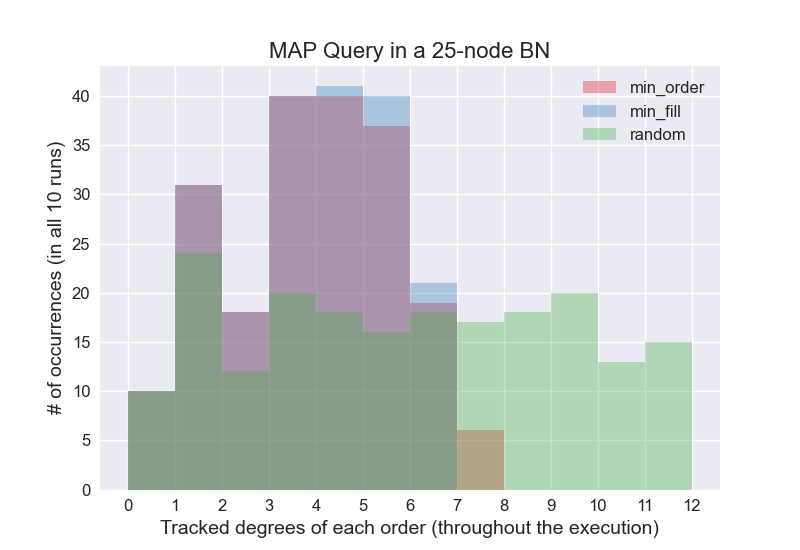
\includegraphics[width=5.2cm]{Assets/map-hist-25nodes.png} }}%
    \qquad
    \subfloat[\centering c ]{{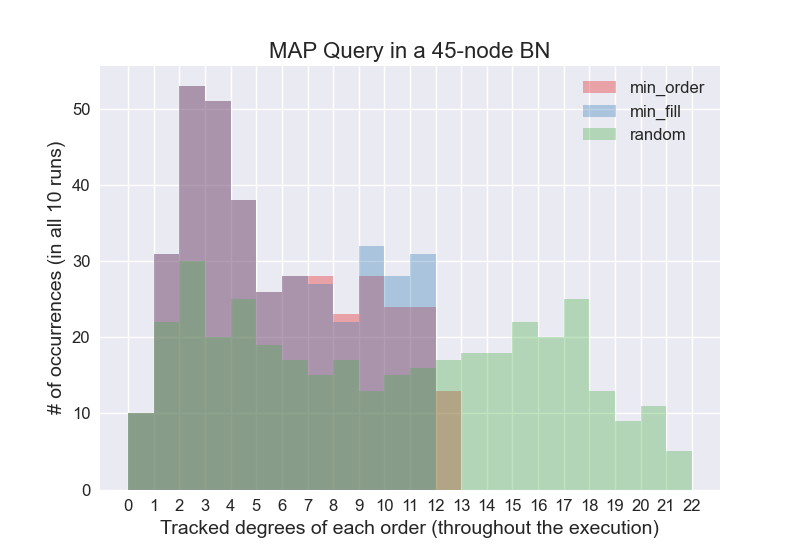
\includegraphics[width=5.2cm]{Assets/map-hist-45nodes.png} }}%
    \qquad
    \caption{MAP Queries }%
    \label{fig:map_histograms}%
\end{figure}
\\\\
In general, the experiment results highlight the superiority of the implemented heuristics over randomness and the importance of the elimination order. The computational complexity decreases in correlation to the quality of the order. 

\section{Modelling the Use Case}
\label{usecase}

\subsection{The Use Case - Occupational strain and Coronary Heart Disease}
Our Use Case was modelled based on existing and established literature on the association between work-related stress, defined as Occupational Strain, and Coronary Heart Disease (CHD). Occupational strain is an example of a psychological risk factor that has become of increasing interest in today's demanding and fast-paced working culture and is situated at the heart of intervention by occupational psychologist for organizations. Occupational Strain has been associated with a wide range of job design-related causes and some of them have been discovered to be related to high risk of CHD. In particular, several studies have demonstrated that both high job demands and low decision latitude, according to the Karasek's "Demand-Control Model", are required to convey increased risk, whereas others have shown that low job control was more important than high job demand and an independent predictor of CHD. Moreover, linked to Siegrist's "Effort-Reward Imbalance Model", the balance between one's perceived or actual effort into the job with one's actual or perceived reward in terms of salary, in other words, a low salary perceived, will influence one's risks of CHD outcomes. Between the physiological and psychological consequences of Job strain, multiple mechanisms underlying the relationship between stress and CHD have to be taken into consideration as possible mediating factors, in our model we gave relevance to high cholesterol, hypertension and maladaptive behaviors, i.g. smoking. ~\cite{ref_article6}

\subsection{The Bayesian Network}

%\noindent
%\begin{figure}[H]
    %\centering
    %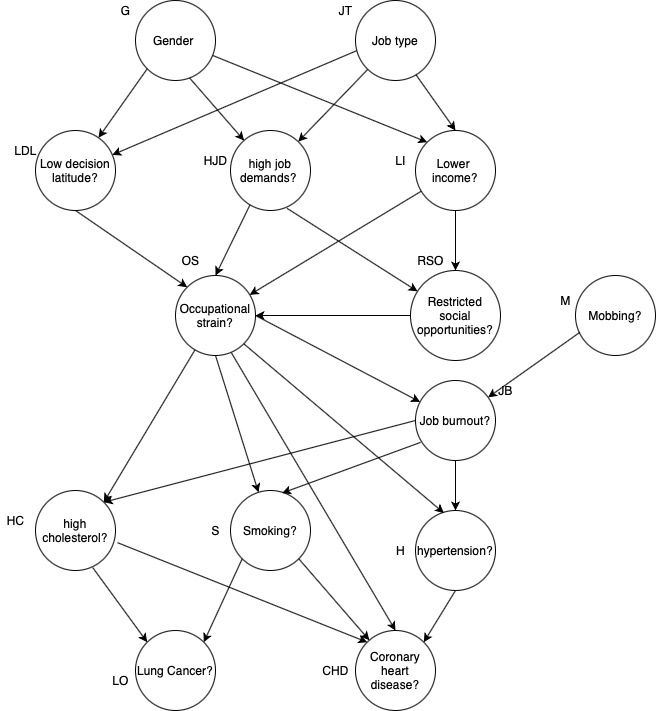
\includegraphics[width=0.8\textwidth]{Assets/BN_diseases.jpg}
    %\caption{BN of the use case}
    %\label{fig:my_label}
%\end{figure}

\subsubsection{Variables:}
\paragraph{Gender (G):} Gender has be selected has a root node with values "Male" and "Female". The reason behind it is that there is a proven distinction between men and women in reported levels of job strain and its consequences, specifically women reported research shows how women typically perceive higher levels of job strain than men. ~\cite{ref_article7}
\paragraph{Job type (JT):} We considered adverse job conditions as our second root node as, like the gender, are know to have an influence on strain levels. We defined active jobs as occupations with high demands combined and high control and passive jobs as low demands and low controls occupations. Both active and passive jobs are related to different maladaptive behaviors (i.g. smoking intensity has been reported as higher in passive jobs). ~\cite{ref_article3}
\paragraph{Mobbing (M):} A third root node was chosen, mobbing (workplace psychological and behavioral aggression) as a possible cause for job burnout.  
\paragraph{Low decision latitude (LDL) and High Job Demands (HJD):} According to the "Demands-Control Model" the combination of low decision-making power and high job requests produce conditions for high job strain. ~\cite{ref_article6}
\paragraph{Lower Income (LI):} According to the "Effort-Reward Imbalance", refers not so much to an income received but an income perceived as lower than due compared to the effort put into the job. ~\cite{ref_article6}
\paragraph{Restricted social Opportunities (RSO):} We considered restricted social opportunities as a secondary variable caused by the low income and which could influence job stress. Social isolation was later added to demand-control scheme ~\cite{ref_article5} as contributing factor to high strain and then proven to increase Cardiovascular Diseases (CVD) prevalence risk ~\cite{ref_article2} 
\paragraph{Occupational Strain (OS):} Job strain can be defined as a state of physical and mental strain caused by an imbalance between strict job requirements and an inadequate ability to adapt and cope ~\cite{ref_article1}. 
\paragraph{Job Burnout (JB):} Job burnout is a state of stress characterized by emotional exhaustion, cynicism, negative self-evaluation and mental disorders. OS is seen as a predecessor of JB. ~\cite{ref_article1}
\paragraph{High Cholesterol (HC), Smoking (S) and Hypertension (H):} We selected these three variables among a frame of possible CHD risk factors which could mediate between occupational strain occurrence. ~\cite{ref_article6}
\paragraph{Coronary heart disease (CHD):} CHD refers to a more specific condition among Cardiovascular Diseases which possible physiological factors risk factors have been linked to psychological imbalances due to a non-favorable work environment.  
\paragraph{Lung Cancer (LC):} This last variable has been added as a possible consequence due to High Cholesterol and Smoking incidence. Cigarette smoking and dietary factors are, in fact, known as dominant risk factors for lung cancer. ~\cite{ref_article8} 

\subsection{Queries}
\subsubsection{Prior marginal:}
As prior marginals we decided to test the probability of being a woman and having a coronary heart disease: Pr(G $\wedge$ CHD).
\\
%table%
\begin{table}
\centering
\caption{Prior marginal}\label{tab1}
\begin{tabular}{p{1.2cm} p{1.2cm} p{1.2cm}}
% \hline
CHD &  G &  Pr\\
\hline
F & {F} & 0.309734\\
F &  {T} & 0.148416\\
T & {F} & 0.352499\\
T & {T} & 0.157501\\
% \hline
\end{tabular}
\end{table}\\
Prior marginal query suggests that females are more likely to be diagnosed with CHD than males in general. On the other hand they are also more likely to be negatively diagnosed than males.
\subsubsection{Posterior marginal:} 
Evidence shows that heavy smokers are more likely to report high job demands ~\cite{ref_article3} . Assuming, as stated above, that smoking behaviors can be a mediating factor between job strain and coronary heart disease we want to test the probability of developing the disease given evidence of this two conditions happening together: Pr(CHD = T $\mid$ S = T, HJD = T).
\\
%table%
\begin{table}
\centering
\caption{Posterior marginal}\label{tab2}
\begin{tabular}{p{1.2cm} p{1.2cm}}
%\hline
CHD &  Pr\\
\hline
F &  0.665808\\
T &  0.334192\\
%\hline
\end{tabular}
\end{table}
\\
It is more likely not to develop a coronary heart disease (66.58\%) than to develop it (33.41\%) given a person is a heavy smoker and more likely to have high job demands. 

\subsubsection{MPE:}
A part from smoking, the other two mediating factors are high cholesterol and hypertension. We want to verify the most likely events to occur knowing that at least one of them or both are true.
\\
%table%
\begin{table}
\centering
\caption{MPE}\label{tab3}
\begin{tabular}{p{0.6cm} p{0.6cm} p{0.6cm}p{0.6cm}p{0.6cm}p{0.6cm}p{0.6cm}p{0.6cm}p{0.6cm}p{0.6cm}p{0.6cm}p{0.6cm}p{0.6cm}p{0.6cm}p{0.6cm}}
%\hline
G & JT & HJD & LI & RSO & M & JB & H & LDL & OS & LC & HC & S & CHD & p
\\
\hline
F & F & T & F & T & F & F & T & F & T & T & T &
   F & F & 0.002031\\
T & F & T & T & F & T & T & F & T & F & F & T & T &
   T & 0.001971\\
T & T & T & T & T & T & T & T & T & F & T & T & T & T & 0.002603\\
%\hline
\end{tabular}
\end{table}
\\
The most likely instantiation of MPE given that a person has a HC or H is when a person has both with a probability of 0.2603\%. Such a person is a male, has an active job high job demands, low income, restricted social opportunities, has experienced mobbing, experienced job burnout, low decision latitude, low occupational strain, has lung cancer, smokes and has a heart coronary disease. 

\subsubsection{MAP:} 
Restricted social opportunities, and so perceived social support, are influenced by the income, which we assume to be different considering the gender and the job type, and can influence the probability of job strain to occur. Given evidence of OS being T and RSO being F we want to verify the most likely instantiations for the G and the JT. \\

%table%
\begin{table}
\centering
\caption{MAP}\label{tab3}
\begin{tabular}{p{1.2cm} p{1.2cm} p{1.2cm}}
%\hline
G & JT & Pr\\
\hline
T & {T} & 0.050574\\
%\hline
\end{tabular}
\end{table}


The MAP query suggest the is most likely to be a man and have and active job type when there are occupational strain and restricted social opportunities present (p = 0.051).

\subsubsection{d-Separation:}
Given evidence of both Occupational strain and mobbing being T, we want to test weather both diseases are independent from the gender and job type.  Therefore, we tested if set of variables {G, J} are d-separated from {CHD, LC} by {OS = T, M = T}. The d-separation proved to be T. 













 
\section{Conclusions and Discussion}

We created a Bayesian Network Reasoner by combining the algorithms d-separation, ordering, network prunning, marginal distributions, MAP, and MPE. The experiment, which tested the average performance of the MAP and MPE algorithms with three different elimination orders, the random order, the min-order, and the min-fill heuristics, revealed that the two heuristics outperformed the random heuristic significantly. \\
The reasoner with the heuristics was used to test our use case based on the correlation between OS and CHD. We tested it for five different queries. According to the prior marginal query, females are more likely than males to be tested positively and negatively for CHD. This could be because females are more likely to report symptoms to their doctor.
The posterior marginal query revealed that if a person is a heavy smoker and has a high job demand, he or she is more likely not to develop coronary heart disease than to develop it. This runs counter to our hypothesis.
According to the MPE query, the most likely instantiation of a person with high cholesterol and hypertension is someone who scores true on almost all the risk variables which is representative of our prediction.
When there is occupational strain and limited social opportunities, the MAP suggests that is most likely to be a man with an active job type.
Given the evidence of both occupational strain and mobbing being true, the d-separation indicated true is independent of gender and job type.


%
% ---- Bibliography ----
%
% BibTeX users should specify bibliography style 'splncs04'.
% References will then be sorted and formatted in the correct style.
%
% \bibliographystyle{splncs04}
% \bibliography{mybibliography}
%

\begin{thebibliography}{8}


\bibitem{ref_article1}
Guan, S., Xiaerfuding, X., Ning, L., Lian, Y., Jiang, Y., Liu, J., & Ng, T. (2017). Effect of Job Strain on Job Burnout, Mental Fatigue and Chronic Diseases among Civil Servants in the Xinjiang Uygur Autonomous Region of China. International Journal of Environmental Research and Public Health, 14(8), 872. \doi{https://doi.org/10.3390/ijerph14080872}

\bibitem{ref_article2}
Johnson, J. V., Hall, E. M., & Theorell, T. (1989). Combined effects of job strain and social isolation on cardiovascular disease morbidity and mortality in a random sample of the Swedish male working population. Scandinavian Journal of Work, Environment & Health, 15(4), 271–279. \doi{https://doi.org/10.5271/sjweh.1852}

\bibitem{ref_article3}
Kouvonen, A., KivimaKi, M., Vaananen, A., Heponiemi, T., Elovainio, M., Ala-Mursula, L., Virtanen, M., Pentti, J., Linna, A., & Vahtera, J. (2007). Job Strain and Adverse Health Behaviors: The Finnish Public Sector Study. Journal of Occupational and Environmental Medicine, 49(1), 68–74. \doi{https://doi.org/10.1097/jom.0b013e31802db54a}

\bibitem{ref_article4}
Kuper, H. (2003). Job strain, job demands, decision latitude, and risk of coronary heart disease within the Whitehall II study. Journal of Epidemiology & Community Health, 57(2), 147–153. \doi{https://doi.org/10.1136/jech.57.2.147}

\bibitem{ref_article5}
Landsbergis, P. A., Schnall, P. L., Deitz, D., Friedman, R., & Pickering, T. (1992). The patterning of psychological attributes and distress by ?job strain? and social support in a sample of working men. Journal of Behavioral Medicine, 15(4), 379–405. \doi{https://doi.org/10.1007/bf00844730}

\bibitem{ref_article6}
Sara, J. D., Prasad, M., Eleid, M. F., Zhang, M., Widmer, R. J., & Lerman, A. (2018). Association Between Work‐Related Stress and Coronary Heart Disease: A Review of Prospective Studies Through the Job Strain, Effort‐Reward Balance, and Organizational Justice Models. Journal of the American Heart Association, 7(9). https://doi.org/10.1161/jaha.117.008073

\bibitem{ref_article7}
Theorell, T., Hammarström, A., Gustafsson, P. E., Magnusson Hanson, L., Janlert, U., & Westerlund, H. (2013). Job strain and depressive symptoms in men and women: a prospective study of the working population in Sweden. Journal of Epidemiology and Community Health, 68(1), 78–82. \doi{https://doi.org/10.1136/jech-2012-202294}

\bibitem{ref_article8}
Ziegler, R. G., Mayne, S. T., & Swanson, C. A. (1996). Nutrition and lung cancer. Cancer Causes and Control, 7(1), 157–177. \doi{https://doi.org/10.1007/bf00115646}
\end{thebibliography}

\newpage
\section{Appendix}

% %table%
% \begin{table}
% \centering
% \caption{Probabilities for Gender (G)}\label{tab1}
% \begin{tabular}{|l|l|}
% \hline
% G &  P\\
% \hline
% F &	0.51\\
% T &	0.49\\
% \hline
% \end{tabular}
% \end{table}

% %table%
% \begin{table}
% \centering
% \caption{Probabilities for job-type (JT)}\label{tab1}
% \begin{tabular}{|l|l|}
% \hline
% JT &  P\\
% \hline
% F &	0.65\\
% T &	0.35\\
% \hline
% \end{tabular}
% \end{table}

% %table%
% \begin{table}
% \centering
% \caption{Probabilities for high job demands (HJD)}\label{tab1}
% \begin{tabular}{|l|l|l|l|}
% \hline
% JT & G & HJD & HJD $\mid$ JT, G \\
% \hline
% F &	F &	F &	0.44\\
% F &	F &	T &	0.55\\
% F &	T &	F &	0.45\\
% F &	T &	T &	0.55\\
% T &	F &	F &	0.61\\
% T &	F &	T &	0.39\\
% T &	T &	F &	0.22\\
% T &	T &	T &	0.78\\
% \hline
% \end{tabular}
% \end{table}

% \begin{table}
% \centering
% \caption{Probabilities for low decision latitude (LDL)}\label{tab1}
% \begin{tabular}{|l|l|l|l|}
% \hline
% JT &  G & LDL & LDL $\mid$ JT, G\\
% \hline
% F &	F &	F &	0.21\\
% F &	F &	T &	0.79\\
% F &	T &	F &	0.41\\
% F &	T &	T &	0.59\\
% T &	F &	F &	0.63\\
% T &	F &	T &	0.27\\
% T &	T &	F &	0.67\\
% T &	T &	T &	0.33\\
% \hline
% \end{tabular}
% \end{table}


% %table%
% \begin{table}
% \centering
% \caption{Probabilities for low income (LI)}\label{tab1}
% \begin{tabular}{|l|l|l|l|}
% \hline
% JT & G &  LI & LI $\mid$ JT, G \\
% \hline
% F &	F &	F &	0.2\\
% F &	F &	T &	0.8\\
% F &	T &	F &	0.31\\
% F &	T &	T &	0.69\\
% T &	F &	F &	0.63\\
% T &	F &	T &	0.37\\
% T &	T &	F &	0.59\\
% T &	T &	T &	0.41\\

% \hline
% \end{tabular}
% \end{table}

% \begin{table}
% \centering
% \caption{Probabilities for restricted social opportunities (RSO)}\label{tab1}
% \begin{tabular}{|l|l|l|l|}
% \hline
% HJD & LI & RSO & RSO $\mid$ HJD, LI\\
% \hline
% F &	F &	F &	0.74\\
% F &	F &	T &	0.26\\
% F &	T &	F &	0.3\\
% F &	T &	T &	0.7\\
% T &	F &	F &	0.34\\
% T &	F &	T &	0.66\\
% T &	T &	F &	0.18\\
% T &	T &	T &	0.82\\
% \hline
% \end{tabular}
% \end{table}


% \begin{table}
% \centering
% \caption{Probabilities for Occupational strain (OS)}\label{tab1}
% \begin{tabular}{|l|l|l|l|l|l|l|}
% \hline
% LDL & HJD & LI & RSO & OS & OS $\mid$ LDL, HJD, LI, RSO\\
% \hline
% F &	F &	F &	F &	F &	0.95\\
% F &	F &	F&	F &	T &	0.05\\
% F &	F &	F &	T &	F &	0.31\\
% F & F &	F &	T &	T &	0.69\\
% F &	F &	T &	F &	F &	0.22\\
% F &	F &	T &	F &	T &	0.78\\
% F &	F & T &	T &	F &	0.2\\
% F &	F &	T &	T &	T &	0.8\\
% F &	T &	F &	F &	F &	0.21\\
% F & T &	F &	F &	T &	0.79\\
% F &	T &	F &	T &	F &	0.17\\
% F &	T &	F &	T &	T &	0.83\\
% F &	T &	T &	F &	F &	0.33\\
% F &	T &	T &	F &	T &	0.67\\
% F &	T &	T &	T &	F &	0.35\\
% F & T &	T &	T &	T & 	0.65\\
% T &	F &	F &	F &	F &	0.25\\
% T &	F &	F &	F &	T &	0.75\\
% T & 	F &	F &	T &	F &	0.32\\
% T &	F &	F &	T &	T &	0.68\\
% T &	F &	T &	F &	F &	0.22\\
% T &	F &	T &	F &	T & 	0.78\\
% T & 	F &	T &	T &	F &	0.29\\
% T &	F &	T &	T &	T &	0.71\\
% T &	T &	F &	F &	F &	0.31\\
% T &	T &	F &	F &	T & 	0.69\\
% T &	T &	F &	T &	F &	0.27\\
% T &	T &	F &	T &	T &	0.73\\
% T &	T &	T &	F &	F &	0.22\\
% T &	T &	T &	F &	T &	0.78\\
% T &	T &	T &	T &	F &	0.11\\
% T &	T &	T &	T &	T &	0.89\\

% \hline
% \end{tabular}
% \end{table}

% %table%
% \begin{table}
% \centering
% \caption{Probabilities for Mobbing (M)}\label{tab1}
% \begin{tabular}{|l|l|}
% \hline
% M &  P\\
% \hline
% F &	0.6\\
% T &	0.4\\
% \hline
% \end{tabular}
% \end{table}


% \begin{table}
% \centering
% \caption{Probabilities for job burnout (JB))}\label{tab1}
% \begin{tabular}{|l|l|l|l|}
% \hline
% OS & M & JB & JB $\mid$ OS, M\\
% \hline
% F &	F &	F &	0.8\\
% F &	F &	T &	0.2\\
% F &	T &	F &	0.22\\
% F &	T &	T &	0.78\\
% T &	F &	F &	0.2\\
% T &	F &	T &	0.8\\
% T &	T &	F &	0.05\\
% T &	T &	T &	0.95\\
% \hline
% \end{tabular}
% \end{table}

% \begin{table}
% \centering
% \caption{Probabilities for high cholesterol (HC))}\label{tab1}
% \begin{tabular}{|l|l|l|l|}
% \hline
% OS & JB & HC & HC $\mid$ OS, JB\\
% \hline
% F &	F &	F &	0.56\\
% F &	F &	T &	0.44\\
% F &	T &	F &	0.15\\
% F &	T &	T &	0.85\\
% T &	F &	F &	0.3\\
% T &	F &	T &	0.7\\
% T &	T &	F &	0.27\\
% T &	T &	T &	0.73\\
% \hline
% \end{tabular}
% \end{table}


% \begin{table}
% \centering
% \caption{Probabilities for smoking (S))}\label{tab1}
% \begin{tabular}{|l|l|l|l|}
% \hline
% OS & JB & S & S $\mid$ OS, JB\\
% \hline
% F &	F &	F &	0.55\\
% F &	F &	T &	0.45\\
% F &	T &	F &	0.2\\
% F &	T &  T &	0.8\\
% T &	F &	F &	0.31\\
% T &	F &	T &	0.69\\
% T &	T &	F &	0.25\\
% T &	T &	T &	0.75\\
% \hline
% \end{tabular}
% \end{table}




% \begin{table}
% \centering
% \caption{Probabilities for hypertension (H)}\label{tab1}
% \begin{tabular}{|l|l|l|l|}
% \hline
% OS & JB & H & H $\mid$ OS, JB\\
% \hline
% F &	F &	F &	0.61\\
% F &	F &	T &	0.39\\
% F &	T &	F &	0.32\\
% F &	T &	T &	0.68\\
% T &	F &	F &	0.25\\
% T &	F &	T &	0.75\\
% T &	T &	F &	0.16\\
% T &	T &	T &	0.84\\
% \hline
% \end{tabular}
% \end{table}

% \begin{table}
% \centering
% \caption{Probabilities for Lung Cancer (LC)}\label{tab1}
% \begin{tabular}{|l|l|l|l|}
% \hline
%  HC & S & LS & LC $\mid$ HC, S\\
% \hline
% F &	F &	F &	0.71\\
% F &	F &	T &	0.29\\
% F &	T &	F &	0.25\\
% F &	T &	T &	0.75\\
% T &	F &	F &	0.37\\
% T &	F &	T &	0.63\\
% T &	T &	F &	0.11\\
% T &	T &	T &	0.89\\
% \hline
% \end{tabular}
% \end{table}

% \begin{table}
% \centering
% \caption{Probabilities for coronary heart disease (CHD)}\label{tab1}
% \begin{tabular}{|l|l|l|l|l|l|}
% \hline
% HC & S & H & OS & CHD & CHD $\mid$ HC, S, H, OS, CHD\\
% \hline
% F &	F &	F &	F &	F &	0.84\\
% F &	F &	F &	F &	T &	0.16\\
% F &	F &	T &	F &	F &	0.42\\
% F &	F &	T &	F &	T &	0.58\\
% F &	F &	F &	T &	F &	0.62\\
% F &	F &	F &	T &	T &	0.38\\
% F &	F &	T &	T &	F &	0.38\\
% F &	F &	T &	T &	T &	0.62\\
% F &	T &	F &	T & 	F &	0.25\\
% F &	T &	F &	F &	F &	0.53\\
% F &	T &	F &	F &	T &	0.47\\
% F &	T &	T &	F &	F &	0.11\\
% F &	T &	T &	F &	T &	0.89\\
% F &	T &	F &	T &	T &	0.75\\
% F &	T &	T &	T &	F &	0.33\\
% F &	T &	T &	T &	T &	0.67\\
% T &	F &	F &	F &	F &	0.46\\
% T &	F &	F &	F &	T &	0.54\\
% T &	F &	T &	F &	F &	0.66\\
% T &	F &	T &	F &	T &	0.34\\
% T &	F &	F &	T &	F &	0.65\\
% T &	F &	F &	T &	T &	0.35\\
% T &	F &	T &	T & F &	0.58\\
% T &	F &	T &	T &	T &	0.42\\
% T &	T &	F & F &	F &	0.32\\
% T &	T &	F &	F &	T &	0.68\\
% T &	T &	T &	F &	F &	0.44\\
% T &	T &	T &  F &	T &	0.56\\
% T &	T &	F &	T &	F &	0.24\\
% T &	T &	F & T &	T &	0.76\\
% T &	T &  T &	T &	F &	0.04\\
% T &	T &	T &	T &	T &	0.96\\
% \hline
% \end{tabular}
% \end{table}


\begin{figure}[H]
    %\centering
    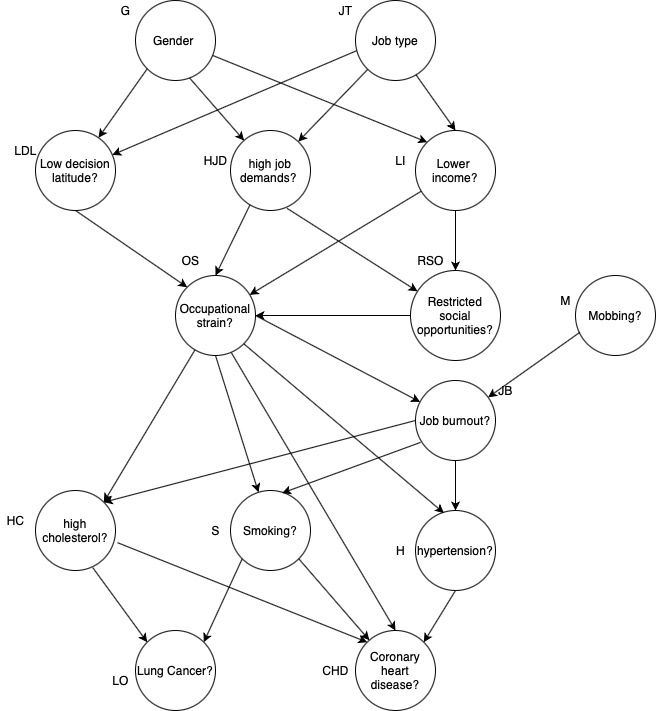
\includegraphics[width= 1.2\textwidth]{Assets/BN_diseases.jpg}
    \caption{BN of the use case}
    \label{fig:my_label}
\end{figure}

%table%
\begin{table}
\centering
\caption{Probabilities for Gender (G)}\label{tab1}
\begin{tabular}{p{1.2cm} p{1.2cm} }
\hline
G &  P\\
\hline
F &	0.51\\
T &	0.49\\
\hline
\end{tabular}
\end{table}

%table%
\begin{table}
\centering
\caption{Probabilities for job-type (JT)}\label{tab1}
\begin{tabular}{p{1.2cm} p{1.2cm} }
\hline
JT &  P\\
\hline
F &	0.65\\
T &	0.35\\
\hline
\end{tabular}
\end{table}

%table%
\begin{table}
\centering
\caption{Probabilities for high job demands (HJD)}\label{tab1}
\begin{tabular}{p{1.2cm} p{1.2cm} p{1.2cm} p{1.5cm} }
\hline
JT & G & HJD & HJD $\mid$ JT, G \\
\hline
F &	F &	F &	0.44\\
F &	F &	T &	0.55\\
F &	T &	F &	0.45\\
F &	T &	T &	0.55\\
T &	F &	F &	0.61\\
T &	F &	T &	0.39\\
T &	T &	F &	0.22\\
T &	T &	T &	0.78\\
\hline
\end{tabular}
\end{table}

\begin{table}
\centering
\caption{Probabilities for low decision latitude (LDL)}\label{tab1}
\begin{tabular}{p{1.2cm} p{1.2cm} p{1.2cm} p{1.5cm} }
\hline
JT &  G & LDL & LDL $\mid$ JT, G\\
\hline
F &	F &	F &	0.21\\
F &	F &	T &	0.79\\
F &	T &	F &	0.41\\
F &	T &	T &	0.59\\
T &	F &	F &	0.63\\
T &	F &	T &	0.27\\
T &	T &	F &	0.67\\
T &	T &	T &	0.33\\
\hline
\end{tabular}
\end{table}


%table%
\begin{table}
\centering
\caption{Probabilities for low income (LI)}\label{tab1}
\begin{tabular}{p{1.2cm} p{1.2cm} p{1.2cm} p{1.5cm} }
\hline
JT & G &  LI & LI $\mid$ JT, G \\
\hline
F &	F &	F &	0.2\\
F &	F &	T &	0.8\\
F &	T &	F &	0.31\\
F &	T &	T &	0.69\\
T &	F &	F &	0.63\\
T &	F &	T &	0.37\\
T &	T &	F &	0.59\\
T &	T &	T &	0.41\\

\hline
\end{tabular}
\end{table}

\begin{table}
\centering
\caption{Probabilities for restricted social opportunities (RSO)}\label{tab1}
\begin{tabular}{p{1.2cm} p{1.2cm} p{1.2cm} p{2.5cm} }
\hline
HJD & LI & RSO & RSO $\mid$ HJD, LI\\
\hline
F &	F &	F &	0.74\\
F &	F &	T &	0.26\\
F &	T &	F &	0.3\\
F &	T &	T &	0.7\\
T &	F &	F &	0.34\\
T &	F &	T &	0.66\\
T &	T &	F &	0.18\\
T &	T &	T &	0.82\\
\hline
\end{tabular}
\end{table}


\begin{table}
\centering
\caption{Probabilities for Occupational strain (OS)}\label{tab1}
\begin{tabular}{p{1.2cm} p{1.2cm} p{1.2cm} p{1.2cm} p{1.2cm} p{2cm} }
\hline
LDL & HJD & LI & RSO & OS & OS $\mid$ LDL, HJD, LI, RSO\\
\hline
F &	F &	F &	F &	F &	0.95\\
F &	F &	F&	F &	T &	0.05\\
F &	F &	F &	T &	F &	0.31\\
F & F &	F &	T &	T &	0.69\\
F &	F &	T &	F &	F &	0.22\\
F &	F &	T &	F &	T &	0.78\\
F &	F & T &	T &	F &	0.2\\
F &	F &	T &	T &	T &	0.8\\
F &	T &	F &	F &	F &	0.21\\
F & T &	F &	F &	T &	0.79\\
F &	T &	F &	T &	F &	0.17\\
F &	T &	F &	T &	T &	0.83\\
F &	T &	T &	F &	F &	0.33\\
F &	T &	T &	F &	T &	0.67\\
F &	T &	T &	T &	F &	0.35\\
F & T &	T &	T &	T & 	0.65\\
T &	F &	F &	F &	F &	0.25\\
T &	F &	F &	F &	T &	0.75\\
T & 	F &	F &	T &	F &	0.32\\
T &	F &	F &	T &	T &	0.68\\
T &	F &	T &	F &	F &	0.22\\
T &	F &	T &	F &	T & 	0.78\\
T & 	F &	T &	T &	F &	0.29\\
T &	F &	T &	T &	T &	0.71\\
T &	T &	F &	F &	F &	0.31\\
T &	T &	F &	F &	T & 	0.69\\
T &	T &	F &	T &	F &	0.27\\
T &	T &	F &	T &	T &	0.73\\
T &	T &	T &	F &	F &	0.22\\
T &	T &	T &	F &	T &	0.78\\
T &	T &	T &	T &	F &	0.11\\
T &	T &	T &	T &	T &	0.89\\

\hline
\end{tabular}
\end{table}

%table%
\begin{table}
\centering
\caption{Probabilities for Mobbing (M)}\label{tab1}
\begin{tabular}{p{1.2cm} p{1.2cm} }
\hline
M &  P\\
\hline
F &	0.6\\
T &	0.4\\
\hline
\end{tabular}
\end{table}


\begin{table}
\centering
\caption{Probabilities for job burnout (JB))}\label{tab1}
\begin{tabular}{p{1.2cm} p{1.2cm} p{1.2cm} p{2cm} }
\hline
OS & M & JB & JB $\mid$ OS, M\\
\hline
F &	F &	F &	0.8\\
F &	F &	T &	0.2\\
F &	T &	F &	0.22\\
F &	T &	T &	0.78\\
T &	F &	F &	0.2\\
T &	F &	T &	0.8\\
T &	T &	F &	0.05\\
T &	T &	T &	0.95\\
\hline
\end{tabular}
\end{table}

\begin{table}
\centering
\caption{Probabilities for high cholesterol (HC))}\label{tab1}
\begin{tabular}{p{1.2cm} p{1.2cm} p{1.2cm} p{2cm} }
\hline
OS & JB & HC & HC $\mid$ OS, JB\\
\hline
F &	F &	F &	0.56\\
F &	F &	T &	0.44\\
F &	T &	F &	0.15\\
F &	T &	T &	0.85\\
T &	F &	F &	0.3\\
T &	F &	T &	0.7\\
T &	T &	F &	0.27\\
T &	T &	T &	0.73\\
\hline
\end{tabular}
\end{table}


\begin{table}
\centering
\caption{Probabilities for smoking (S))}\label{tab1}
\begin{tabular}{p{1.2cm} p{1.2cm} p{1.2cm} p{2.2cm} }
\hline
OS & JB & S & S $\mid$ OS, JB\\
\hline
F &	F &	F &	0.55\\
F &	F &	T &	0.45\\
F &	T &	F &	0.2\\
F &	T &  T &	0.8\\
T &	F &	F &	0.31\\
T &	F &	T &	0.69\\
T &	T &	F &	0.25\\
T &	T &	T &	0.75\\
\hline
\end{tabular}
\end{table}




\begin{table}
\centering
\caption{Probabilities for hypertension (H)}\label{tab1}
\begin{tabular}{p{1.2cm} p{1.2cm} p{1.2cm} p{2cm} }
\hline
OS & JB & H & H $\mid$ OS, JB\\
\hline
F &	F &	F &	0.61\\
F &	F &	T &	0.39\\
F &	T &	F &	0.32\\
F &	T &	T &	0.68\\
T &	F &	F &	0.25\\
T &	F &	T &	0.75\\
T &	T &	F &	0.16\\
T &	T &	T &	0.84\\
\hline
\end{tabular}
\end{table}

\begin{table}
\centering
\caption{Probabilities for Lung Cancer (LC)}\label{tab1}
\begin{tabular}{p{1.2cm} p{1.2cm} p{1.2cm} p{2cm} }
\hline
 HC & S & LS & LC $\mid$ HC, S\\
\hline
F &	F &	F &	0.71\\
F &	F &	T &	0.29\\
F &	T &	F &	0.25\\
F &	T &	T &	0.75\\
T &	F &	F &	0.37\\
T &	F &	T &	0.63\\
T &	T &	F &	0.11\\
T &	T &	T &	0.89\\
\hline
\end{tabular}
\end{table}

\begin{table}
\centering
\caption{Probabilities for coronary heart disease (CHD)}\label{tab1}
\begin{tabular}{p{1.2cm} p{1.2cm} p{1.2cm} p{1.2cm} p{1.2cm} p{2cm} }
\hline
HC & S & H & OS & CHD & CHD $\mid$ HC, S, H, OS, CHD\\
\hline
F &	F &	F &	F &	F &	0.84\\
F &	F &	F &	F &	T &	0.16\\
F &	F &	T &	F &	F &	0.42\\
F &	F &	T &	F &	T &	0.58\\
F &	F &	F &	T &	F &	0.62\\
F &	F &	F &	T &	T &	0.38\\
F &	F &	T &	T &	F &	0.38\\
F &	F &	T &	T &	T &	0.62\\
F &	T &	F &	T & 	F &	0.25\\
F &	T &	F &	F &	F &	0.53\\
F &	T &	F &	F &	T &	0.47\\
F &	T &	T &	F &	F &	0.11\\
F &	T &	T &	F &	T &	0.89\\
F &	T &	F &	T &	T &	0.75\\
F &	T &	T &	T &	F &	0.33\\
F &	T &	T &	T &	T &	0.67\\
T &	F &	F &	F &	F &	0.46\\
T &	F &	F &	F &	T &	0.54\\
T &	F &	T &	F &	F &	0.66\\
T &	F &	T &	F &	T &	0.34\\
T &	F &	F &	T &	F &	0.65\\
T &	F &	F &	T &	T &	0.35\\
T &	F &	T &	T & F &	0.58\\
T &	F &	T &	T &	T &	0.42\\
T &	T &	F & F &	F &	0.32\\
T &	T &	F &	F &	T &	0.68\\
T &	T &	T &	F &	F &	0.44\\
T &	T &	T &  F &	T &	0.56\\
T &	T &	F &	T &	F &	0.24\\
T &	T &	F & T &	T &	0.76\\
T &	T &  T &	T &	F &	0.04\\
T &	T &	T &	T &	T &	0.96\\
\hline
\end{tabular}
\end{table}



\end{document}


